\documentclass[10pt,fleqn]{article} % Default font size and left-justified equations
\usepackage[%
    pdftitle={SLCI : Modélisation par schéma blocs},
    pdfauthor={Xavier Pessoles}]{hyperref}
    
\input{style/new_style}
\input{style/macros_SII}
\usepackage{style/schemabloc}
\usepackage{multicol}
%\fichetrue
%\fichefalse

\proftrue
%\proffalse

\tdtrue
%\tdfalse

\courstrue
\coursfalse

\def\discipline{Sciences \\Industrielles de \\ l'Ingénieur}
\def\xxtete{Sciences Industrielles de l'Ingénieur}

\def\classe{PTSI}
\def\xxnumpartie{Partie 2}
\def\xxpartie{Découverte des Systèmes Linéaires Continus et Invariants\\
Analyse, Modélisation, Résolution}

\def\xxnumchapitre{Chapitre 3}
\def\xxchapitre{Modélisation des SLCI par schémas blocs}

\def\xxtitreexo{Transmission à variation continue vario-fendt}
\def\xxsourceexo{\hspace{.2cm} D'après concours CCP MP -- 2008.}


\def\xxposongletx{2}
\def\xxposonglettext{1.45}
\def\xxposonglety{20}
\def\xxonglet{Part. 2 -- Ch. 3}

\def\xxactivite{TD 4}
\def\xxauteur{\textsl{Xavier Pessoles}}

\def\xxcompetences{%
\textsl{%
\textbf{Savoirs et compétences :}\\
%\noindent \textbf{Résoudre :} à partir des modèles retenus :
%\begin{itemize}[label=\ding{112},font=\color{ocre}] 
%\item choisir une méthode de résolution analytique, graphique, numérique;
%\item mettre en \oe{}uvre une méthode de résolution.
%\end{itemize}
%\begin{itemize}[label=\ding{112},font=\color{ocre}] 
%\item \textit{Rés -- C1.1 :} Loi entrée sortie géométrique et cinématique -- Fermeture géométrique.
%\end{itemize}
%
%\noindent \textit{Mod2 -- C4.1 :} Représentation par schéma bloc.
}}

\def\xxfigures{\includegraphics[width=.8\textwidth]{images/Tracteur}
}%figues de la page de garde

\def\xxpied{%
Partie 2 -- Découverte des SLCI\\
Ch. 3 : Modélisation par schémas blocs -- \xxactivite%
}


\setcounter{secnumdepth}{5}
%---------------------------------------------------------------------------


\begin{document}
%\chapterimage{png/Fond_Cin}
\input{style/new_pagegarde}
\vspace{10cm}
\pagestyle{fancy}
\thispagestyle{plain}


\def\columnseprulecolor{\color{ocre}}
\setlength{\columnseprule}{0.4pt} 
\begin{multicols}{2}

\ifprof
\else
\fi
\subsection*{Mise en situation}
\begin{obj} 
%Dans le but de valider le moteur électrique utilisé sur la prothèse ainsi que la structure mécanique, on cherche à valider l'exigence 1.3.1.
\end{obj}
Les tracteurs de la gamme \textit{Fendrt 900 Vario} sont équipés d'une transmission à variation continue. Ce dispositif permet de régler la vitesse de façon continue sans à-coups et d'exploiter au mieux les capacités du moteur thermique quelle que soit la configuration de travail. Pour cela le tracteur est équipé d'un groupe hydraulique constitué d'un arbre de commande, de deux moteurs hydrauliques ainsi que d'une pompe à débit variable.
\begin{center}
\includegraphics[width=.48\textwidth]{images/req}
\end{center}

\begin{center}
\includegraphics[width=.48\textwidth]{images/ibd.pdf}
\end{center}

\subsection*{Asservissement de position de l'arbre de commande}
Afin de régler le débit de la pompe, on actionne un arbre de commande à l'aide d'un moteur à courant continu dont les équations caractéristiques sont les suivantes : 
\begin{itemize}
\item $u(t) = Ri(t)+e(t)$;
\item $e(t)=k_e \dfrac{\text{d}\theta(t)}{\text{d}t}$;
\item $c(t)=k_a i(t)$;
\item $J_e \cdot \dfrac{\text{d}^2\theta(t)}{\text{d}t^2} = c(t)$.
\end{itemize}

Le moteur est asservi en vitesse grâce à une génératrice tachymétrique de gain $K_t$.

Le moteur est aussi asservi en position. On utilise pour cela  un capteur de gain $K_p$ fournissant une tension $u_r(t)$ proportionnel à la position angulaire de l'arbre moteur. Le signal de commande est élaboré après que l'écart $\varepsilon(t)$ a été modulé par un correcteur proportionnel de gain $K_C$. Ainsi, on a :
\begin{itemize}
\item $u(t)=K_c \left(u_e(t)-u_r(t)\right)$.
\end{itemize}

Le moteur à courant continu entraîne un arbre de commande comportant deux cames destinées à commander la pompe ainsi que deux moteurs hydrauliques (dont le but est de fournir de l'énergie hydraulique au système). 


\subparagraph{}
\textit{Donner les équations du moteur à courant continu dans le domaine de Laplace et tracer les schémas blocs élémentaires correspondant. Réaliser alors le schéma bloc du moteur à courant continu.}
\begin{corrige}
On a les équations suivantes : 
\begin{itemize}
\item $U(p) = RI(p)+E(p)$;
\item $E(p)=k_e p\Theta(p)$;
\item $C(p)=k_a I(p)$;
\item $J_e p^2\Theta(p) = C(p)$.
\end{itemize}
On peut ainsi établir les schémas blocs suivants :


\noindent \footnotesize{
\begin{tabular}{cc}
\begin{tikzpicture}
\sbEntree{E}

\sbBloc[4]{blocA}{$k_e p$}{E}
    \sbRelier[$\Theta(p)$]{E}{blocA}

\sbSortie{S}{blocA}
    \sbRelier{blocA}{S}
    \sbNomLien[0.8]{S}{$E(p)$}
\end{tikzpicture}
 &
\begin{tikzpicture}
\sbEntree{E}

\sbBloc[4]{blocA}{$k_a$}{E}
    \sbRelier[$I(p)$]{E}{blocA}

\sbSortie{S}{blocA}
    \sbRelier{blocA}{S}
    \sbNomLien[0.8]{S}{$C(p)$}
\end{tikzpicture}
 \\
\begin{tikzpicture}
\sbEntree{E}

\sbBloc[4]{blocA}{$\dfrac{1}{J_e p^2}$}{E}
    \sbRelier[$C(p)$]{E}{blocA}

\sbSortie{S}{blocA}
    \sbRelier{blocA}{S}
    \sbNomLien[0.8]{S}{$\Theta(p)$}
\end{tikzpicture}
&
\begin{tikzpicture}
\sbEntree{E}

\sbComp{c1}{E}
    \sbRelier[$U(p)$]{E}{c1}
    
\sbBloc{b1}{$\dfrac{1}{R}$}{c1}
    \sbRelier{c1}{b1}

\sbSortie{S}{b1}
    \sbRelier{b1}{S}
    \sbNomLien[0.8]{S}{$I(p)$}
    
\sbDecaleNoeudy{c1}{n1}
    \sbRelier[$E(p)$]{n1}{c1}

\end{tikzpicture}
 \\
\end{tabular}}


\begin{center}
\begin{tikzpicture}
\sbEntree{E}

\sbComp{c1}{E}
    \sbRelier[$U(p)$]{E}{c1}
    
\sbBloc{b1}{$\dfrac{1}{R}$}{c1}
    \sbRelier{c1}{b1}

\sbBloc{b2}{$k_a$}{b1}
    \sbRelier{b1}{b2}

\sbBloc{b3}{$\dfrac{1}{J_e p^2}$}{b2}
    \sbRelier{b2}{b3}
    
\sbSortie{S}{b3}
    \sbRelier{b3}{S}
    \sbNomLien[0.8]{S}{$\Theta(p)$}
    
\sbDecaleNoeudy{b3}{n1}

\sbBlocr{r1}{$k_e p$}{n1}
    \sbRelierxy{r1}{c1}
    \sbRelieryx{b3-S}{r1}

\end{tikzpicture}
\end{center}

\end{corrige}

On note $M(p)=\dfrac{\Theta(p)}{U(p)}$.

\subparagraph{}
\textit{Réaliser le schéma bloc de l'asservissement en vitesse grâce à la génératrice tachymétrique puis l'asservissement en position en utilisant le correcteur proportionnel et le capteur de position angulaire. Compléter le schéma bloc pour que la grandeur asservie soit l'angle de l'arbre de commande.}
\begin{corrige}
Le signal en sortie du moteur étant une position angulaire, il est nécessaire d'avoir recours à une dérivation pour réaliser le retour tachymétrique. Cela explique donc la présence d'une multiplication par $p$ dans la boucle d'asservissement en vitesse.

Pour que la grandeur asservie soit un angle, on ajoute en entrée du schéma bloc un gain d'adaptation permettant de convertir un angle de consigne en tension de commande.

\footnotesize{
\begin{center}
\begin{tikzpicture}
\sbEntree{E}

\sbBloc{b1}{$K_{adapt}$}{E}
    \sbRelier{E}{b1}
    
\sbComp{c1}{b1}
    \sbRelier{b1}{c1}
    
\sbBloc{b2}{$K_c$}{c1}
    \sbRelier{c1}{b2}

\sbComp{c2}{b2}
    \sbRelier{b2}{c2}

\sbBloc{b3}{$M(p)$}{c2}
    \sbRelier{c2}{b3}
        
\sbSortie[7]{S}{b3}
    \sbRelier{b3}{S}
    \sbNomLien[0.8]{S}{$\Theta(p)$}
    
\sbDecaleNoeudy[4]{b3}{n1}
\sbDecaleNoeudx[4]{b3}{n2}
\sbDecaleNoeudy[8]{b3}{n3}
\sbDecaleNoeudx[6]{b3}{n4}

\sbBlocr[-1.5]{r1}{$K_T p$}{n1}
    \sbRelieryx{n2}{r1}
    %\sbRenvoi{b3-n2}{r1}{}
    \sbRelierxy{r1}{c2}

\sbBlocr{r2}{$K_P$}{n3}
    \sbRelieryx{n4}{r2}
    \sbRelierxy{r2}{c1}
%    \sbrenvoi
%
%\sbDecaleNoeudx{b3}{n3}
%
%\sbBlocr{r1}{$k_e p$}{n1}
%    \sbRelierxy{r1}{c2}
%    \sbRelieryx{n3}{r1}
%  
%
%\sbDecaleNoeudy[8]{c2}{n2}
% \sbBlocr{r2}{$Kpos$}{n2}
%    \sbRelierxy{r2}{c1}
%    \sbRelieryx{n3}{r2}
\end{tikzpicture}
\end{center}}

\end{corrige}


\subparagraph{}
\textit{Une simulation correspondant à une sollicitation par un échelon d'un radian a été réalisée grâce à un logiciel de simulation multiphysique. L'asservissement de la position de l'arbre de commande respecte-t-il les exigences ** et ** du cahier des charges ?}
\begin{center}
\includegraphics[width=.45\textwidth]{images/simulation}
\end{center}

\begin{corrige}

\end{corrige}


\subsection*{Suite}

Sous l'action d'une rotation d'angle $\theta$ de l'arbre de commande, la came de pas $p_p$ provoque une translation $x_{P1}$ d'un galet provoquant lui même le déplacement $x_{P2}$ du distributeur. On note $x_{P2}=x_{P21}-x_{P22}$.

Le débit volumique $q_P(t)$ en sortie du distributeur est proportionnel au déplacement $x_{P2}$ du tiroir : 
\begin{itemize}
\item $q_P(t)=K_d x_{P2}(t)$.
\end{itemize}

En circulant dans le distributeur, le fluide agit sur les vérins dont la vitesse de déplacement est proportionnel à leur section : 
\begin{itemize}
\item $y_{P5}(t)= S \dfrac{\text{d}y_{P5}(t)}{\text{d}t}$.
\end{itemize}


Le vérin permet alors de régler le débit de la pompe en modifiant l'inclinaison $\alpha$ du barillet.


\subparagraph{}
\textit{En faisant l'hypothèse des petits déplacements, donner la relation géométrique entre le déplacement $x_{P21}$ et $x_{P1}$.}
\begin{corrige}

\end{corrige}

\subparagraph{}
\textit{Donner les relations géométriques entre $y_{P5}(t)$ et $\alpha(t)$ puis entre $y_{P3}(t)$ et $\alpha(t)$.}
\begin{corrige}

\end{corrige}

\subparagraph{}
\textit{Compléter alors le schéma bloc de la figure ** traduisant la relation entre la rotation du moteur $\theta(t)$ et la rotation $\alpha(t)$ du barillet permettant le changement de débit de la pompe.}
\begin{corrige}

\end{corrige}

\subparagraph{}
\textit{Compléter alors le schéma bloc de la figure ** traduisant la relation entre la rotation du moteur $\theta(t)$ et la rotation $\alpha(t)$ du barillet permettant le changement de débit de la pompe.}
\begin{corrige}

\end{corrige}

\end{multicols}

\end{document}


